\documentclass[12pt]{amsart}

\addtolength{\hoffset}{-2.25cm}
\addtolength{\textwidth}{4.5cm}
\addtolength{\voffset}{-2.5cm}
\addtolength{\textheight}{5cm}
\setlength{\parskip}{0pt}
\setlength{\parindent}{15pt}
\usepackage{listings}
\usepackage{amsthm}
\usepackage{amsmath}
\usepackage[spanish]{babel}
\usepackage[sort&compress, numbers]{natbib}
\usepackage{amssymb}
\usepackage[utf8]{inputenc}
\usepackage[colorlinks = true, linkcolor = thistle, citecolor = thistle, final]{hyperref}
\usepackage{listings}
\usepackage{ragged2e}
\usepackage{subcaption} 
\usepackage{minted}
\usemintedstyle{borland}
\usepackage{multicol}
\usepackage{listings}
\usepackage{xcolor}
\usepackage{graphicx}
\usepackage[sort&compress, numbers]{natbib}
\usepackage{xcolor}
\usepackage{listings}
\usepackage{ragged2e}
\usepackage{graphicx}
\usepackage[sort&compress, numbers]{natbib}
\usepackage{xcolor}
\usepackage{listings}
\usepackage{ragged2e}
\hypersetup{
    colorlinks=true,
    linkcolor=violet,
    filecolor=violet,     
    urlcolor=violet,
    citecolor=violet,
}
\usepackage{graphicx}
\usepackage[sort&compress, numbers]{natbib}
\usepackage{xcolor}
\usepackage{listings}
\usepackage{ragged2e}

\lstset{style=mystyle}
\usepackage{graphicx}
\usepackage{multicol}
\usepackage{ marvosym }
\newcommand{\ds}{\displaystyle}


\pagestyle{myheadings}

\setlength{\parindent}{0in}
\begin{document}

\pagestyle{empty}



\thispagestyle{empty}

{\scshape Simulación} \hfill {\scshape \Large Tarea 7: Búsqueda local} \hfill  {\scshape 14/Abr/2021}
\author{C. María Montemayor Palos}
\maketitle

\hrule
\hrule
\bigskip
\section{Objetivo}
Examinar y encontrar el máximo local de la función 
\begin{align*}
f(x,y) &= 5e^{(-(0.8y + 1)^2)-(0.8x)^2}(0.8x-1)^2 - \frac{1}{3}\cdot e^{-(0.8x+1)^2-(0.8y)^2}\\ &+e^{-(0.8x)^2-(0.8y)^2}(10(0.8x)^3-2(0.8x)+10(0.8y)^5)
\end{align*}
con restricciones $ -3 \leq x, y \leq 3 \ $. La figura \ref{fig1} muestra la función en tres dimensiones (3D) y dos dimensiones (2D).

\begin{figure}[h!]
\centering
\begin{subfigure}[H]{0.4\linewidth}
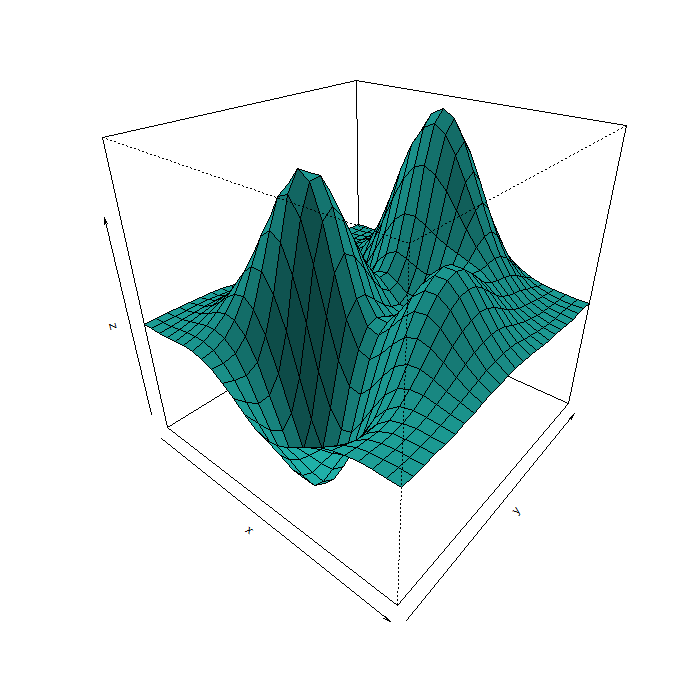
\includegraphics[width=\linewidth]{t7_2d.png}
\caption{}
\label{1a}
\end{subfigure}
\begin{subfigure}[H]{0.4\linewidth}
\includegraphics[width=\linewidth]{grafico2D20.png}
\caption{}
\label{1b}
\end{subfigure}
\caption{Gráficas de la función.}
\label{fig1}
\end{figure}

\section{Metodología}
Para efectos de la tarea \cite{dra} se utiliza el programa R versión 4.0.4 \cite{R} para Windows. Se maximiza la variante de la función bidimensional g(x, y) con las restricciones anteriormente mencionadas, en donde la posición actual es un par $x, y$ y se ocupan dos movimientos aleatorios, $\Delta x$ y $\Delta y$ cuyas combinaciones posibles proveen ocho posiciones vecino, de los cuales aquella que logra el mayor valor para $g$ es seleccionado. Se recurre a una visualización en 2D (como se muestra en la figura \ref{fig2}) debido a que en 3D de limita la visibilidad de los puntos generados.

\clearpage
\section{Código}
Se modifica el código de Schaeffer \cite{codigo} y se mejora la calidad del gráfico en apoyo del repositorio de Vázquez \cite{vazquez}. A continuación se muestra la parte del código donde se encuentra la función \texttt{replica}.
\renewcommand{\listingscaption}{Código}
\begin{listing}[H]
  \begin{minted}[linenos,mathescape,texcl]{clojure}
low <- -3
high <- 3
step <- 0.25
replicas <- 15
replica <- function(t){
  curr <- c(runif(1, low, high), runif(1, low, high))
  best <- curr
  for (tiempo in 1:t) {
    delta <- runif(1, 0, step)
    x1 <- curr + c(-delta,0)  #izquierda
    x2 <- curr + c(delta,0)   #derecha
    y1 <- curr + c(0,-delta)  #arriba
    y2 <- curr + c(0,delta)   #abajo
    
    puntos <- c(x1,x2,y1,y2)
    for(k in 1:8){
      if(puntos[k] < (-3)){
        puntos[k] <- puntos[k]+3 
      }
      if(puntos[k] > 3){
        puntos[k] <- puntos[k]-3
      }
    }
    vx <- c()
    vy <- c()
    for(p in 1:8){
      if(p %% 2 == 0){
        vy <- c(vy,puntos[p])
      }else{
        vx <- c(vx,puntos[p])
      }
    }
    vg <- c()
    for(q in 1:4){
      vg <- c(vg, g(vx[q], vy[q]) )
    }
    dm <- which.max(vg)
    curr <- c(vx[dm], vy[dm])
    if(g(curr[1],curr[2]) > g(best[1],best[2])){
      best <- curr
    }
  }
  return(best)
}
  \end{minted}
  \label{codigo1}
\end{listing}
\clearpage

\section{Resultados y discusión}
En la figura \ref{fig2} se muestran los resultados obtenidos siendo los círculos blancos obtenidos de las 40 réplicas para los 15 pasos. El punto rojo mostrado en las figuras es el punto al que le corresponde el valor máximo de todas las réplicas generadas. El gif de las gráficas se muestra en el repositorio de Montemayor \cite{mtyor}.
\begin{figure}[h!]
\centering
\begin{subfigure}[b]{0.4\linewidth}
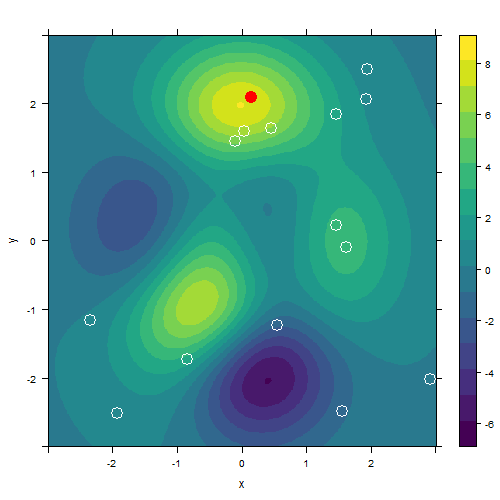
\includegraphics[width=\linewidth]{t7_1.png}
\caption{Paso 1.}
\label{a}
\end{subfigure}
\begin{subfigure}[b]{0.4\linewidth}
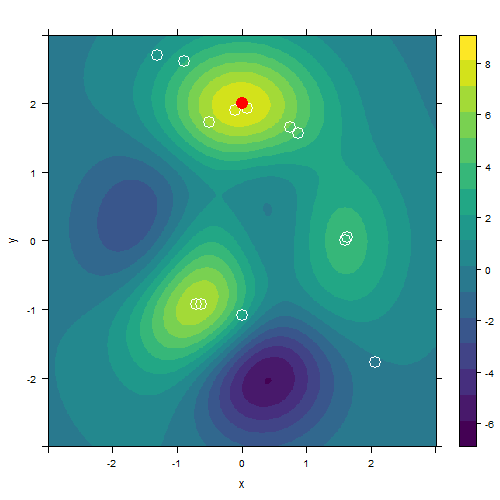
\includegraphics[width=\linewidth]{t7_10.png}
\caption{Paso 10.}
\label{b}
\end{subfigure}
\begin{subfigure}[b]{0.4\linewidth}
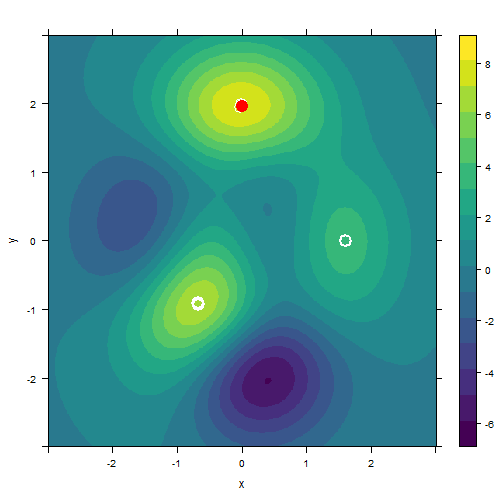
\includegraphics[width=\linewidth]{t7_30.png}
\caption{Paso 30.}
\label{c}
\end{subfigure}
\begin{subfigure}[b]{0.4\linewidth}
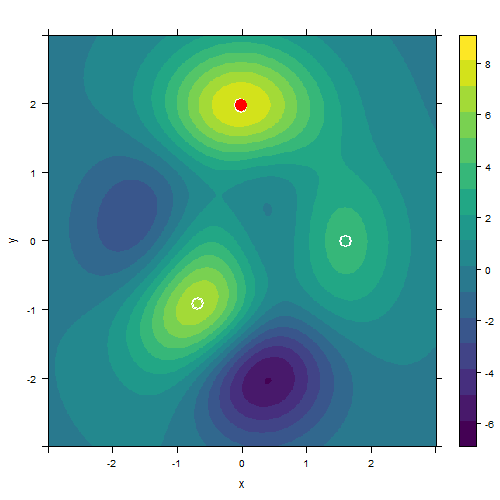
\includegraphics[width=\linewidth]{t7_40.png}
\caption{Paso 40.}
\label{d}
\end{subfigure}
\caption{Búsqueda local de la función.}
\label{fig2}
\end{figure}


\section{Conclusión}
Como es de esperarse, en la figura \ref{a} y \ref{b} se muestra una mayor dispersión de los puntos en cuanto al acercamiento del punto máximo, mientras que en las figuras \ref{c} y \ref{d} tienden a irse a los puntos más altos de la función, esto también depende del pico alto más cercano que esté del punto generado al azar.

\clearpage
\bibliography{referencias}
\bibliographystyle{plainnat}


\end{document}